\documentclass[8pt]{beamer}

% Beamer style
%\usetheme[secheader]{Madrid}
% \usetheme{CambridgeUS}
\useoutertheme{infolines}
\usecolortheme[rgb={0.65,0.15,0.25}]{structure}
% \usefonttheme[onlymath]{serif}
\beamertemplatenavigationsymbolsempty
%\AtBeginSubsection

% Packages
%\usepackage[french]{babel}
\usepackage[latin1]{inputenc}
\usepackage{color}
\usepackage{xspace}
\usepackage{dsfont, stmaryrd}
\usepackage{amsmath, amsfonts, amssymb, stmaryrd}
\usepackage{epsfig}
\usepackage{tikz}
\usepackage{url}
% \usepackage{ulem}
\usepackage{/home/robin/LATEX/Biblio/astats}
%\usepackage[all]{xy}
\usepackage{graphicx}
\usepackage{rotating}
\usepackage{xspace}

% Maths
% \newtheorem{theorem}{Theorem}
% \newtheorem{definition}{Definition}
\newtheorem{proposition}{Proposition}
% \newtheorem{assumption}{Assumption}
% \newtheorem{algorithm}{Algorithm}
% \newtheorem{lemma}{Lemma}
% \newtheorem{remark}{Remark}
% \newtheorem{exercise}{Exercise}
% \newcommand{\propname}{Prop.}
% \newcommand{\proof}{\noindent{\sl Proof:}\quad}
% \newcommand{\eproof}{$\blacksquare$}

% \setcounter{secnumdepth}{3}
% \setcounter{tocdepth}{3}
\newcommand{\pref}[1]{\ref{#1} p.\pageref{#1}}
\newcommand{\qref}[1]{\eqref{#1} p.\pageref{#1}}

% Colors : http://latexcolor.com/
\definecolor{darkred}{rgb}{0.65,0.15,0.25}
\definecolor{darkgreen}{rgb}{0,0.4,0}
\definecolor{darkred}{rgb}{0.65,0.15,0.25}
\definecolor{amethyst}{rgb}{0.6, 0.4, 0.8}
\definecolor{asparagus}{rgb}{0.53, 0.66, 0.42}
\definecolor{applegreen}{rgb}{0.55, 0.71, 0.0}
\definecolor{awesome}{rgb}{1.0, 0.13, 0.32}
\definecolor{blue-green}{rgb}{0.0, 0.87, 0.87}
\definecolor{red-ggplot}{rgb}{0.52, 0.25, 0.23}
\definecolor{green-ggplot}{rgb}{0.42, 0.58, 0.00}
\definecolor{purple-ggplot}{rgb}{0.34, 0.21, 0.44}
\definecolor{blue-ggplot}{rgb}{0.00, 0.49, 0.51}

% Commands
\newcommand{\backupbegin}{
   \newcounter{finalframe}
   \setcounter{finalframe}{\value{framenumber}}
}
\newcommand{\backupend}{
   \setcounter{framenumber}{\value{finalframe}}
}
\newcommand{\emphase}[1]{\textcolor{darkred}{#1}}
\newcommand{\comment}[1]{\textcolor{gray}{#1}}
\newcommand{\paragraph}[1]{\textcolor{darkred}{#1}}
\newcommand{\refer}[1]{{\small{\textcolor{gray}{{\cite{#1}}}}}}
\newcommand{\Refer}[1]{{\small{\textcolor{gray}{{[#1]}}}}}
\newcommand{\goto}[1]{{\small{\textcolor{blue}{[\#\ref{#1}]}}}}
\renewcommand{\newblock}{}

\newcommand{\tabequation}[1]{{\medskip \centerline{#1} \medskip}}
% \renewcommand{\binom}[2]{{\left(\begin{array}{c} #1 \\ #2 \end{array}\right)}}

% Variables 
\newcommand{\Abf}{{\bf A}}
\newcommand{\Beta}{\text{B}}
\newcommand{\Bcal}{\mathcal{B}}
\newcommand{\Bias}{\xspace\mathbb B}
\newcommand{\Cor}{{\mathbb C}\text{or}}
\newcommand{\Cov}{{\mathbb C}\text{ov}}
\newcommand{\cl}{\text{\it c}\ell}
\newcommand{\Ccal}{\mathcal{C}}
\newcommand{\cst}{\text{cst}}
\newcommand{\Dcal}{\mathcal{D}}
\newcommand{\Ecal}{\mathcal{E}}
\newcommand{\Esp}{\xspace\mathbb E}
\newcommand{\Espt}{\widetilde{\Esp}}
\newcommand{\Covt}{\widetilde{\Cov}}
\newcommand{\Ibb}{\mathbb I}
\newcommand{\Fcal}{\mathcal{F}}
\newcommand{\Gcal}{\mathcal{G}}
\newcommand{\Gam}{\mathcal{G}\text{am}}
\newcommand{\Hcal}{\mathcal{H}}
\newcommand{\Jcal}{\mathcal{J}}
\newcommand{\Lcal}{\mathcal{L}}
\newcommand{\Mt}{\widetilde{M}}
\newcommand{\mt}{\widetilde{m}}
\newcommand{\Nbb}{\mathbb{N}}
\newcommand{\Mcal}{\mathcal{M}}
\newcommand{\Ncal}{\mathcal{N}}
\newcommand{\Ocal}{\mathcal{O}}
\newcommand{\pt}{\widetilde{p}}
\newcommand{\Pt}{\widetilde{P}}
\newcommand{\Pbb}{\mathbb{P}}
\newcommand{\Pcal}{\mathcal{P}}
\newcommand{\Qcal}{\mathcal{Q}}
\newcommand{\qt}{\widetilde{q}}
\newcommand{\Rbb}{\mathbb{R}}
\newcommand{\Sbb}{\mathbb{S}}
\newcommand{\Scal}{\mathcal{S}}
\newcommand{\st}{\widetilde{s}}
\newcommand{\St}{\widetilde{S}}
\newcommand{\Tcal}{\mathcal{T}}
\newcommand{\todo}{\textcolor{red}{TO DO}}
\newcommand{\Ucal}{\mathcal{U}}
\newcommand{\Un}{\math{1}}
\newcommand{\Vcal}{\mathcal{V}}
\newcommand{\Var}{\mathbb V}
\newcommand{\Vart}{\widetilde{\Var}}
\newcommand{\Zcal}{\mathcal{Z}}

% Symboles & notations
\newcommand\independent{\protect\mathpalette{\protect\independenT}{\perp}}\def\independenT#1#2{\mathrel{\rlap{$#1#2$}\mkern2mu{#1#2}}} 
\renewcommand{\d}{\text{\xspace d}}
\newcommand{\gv}{\mid}
\newcommand{\ggv}{\, \| \, }
% \newcommand{\diag}{\text{diag}}
\newcommand{\card}[1]{\text{card}\left(#1\right)}
\newcommand{\trace}[1]{\text{tr}\left(#1\right)}
\newcommand{\matr}[1]{\boldsymbol{#1}}
\newcommand{\matrbf}[1]{\mathbf{#1}}
\newcommand{\vect}[1]{\matr{#1}} %% un peu inutile
\newcommand{\vectbf}[1]{\matrbf{#1}} %% un peu inutile
\newcommand{\trans}{\intercal}
\newcommand{\transpose}[1]{\matr{#1}^\trans}
\newcommand{\crossprod}[2]{\transpose{#1} \matr{#2}}
\newcommand{\tcrossprod}[2]{\matr{#1} \transpose{#2}}
\newcommand{\matprod}[2]{\matr{#1} \matr{#2}}
\DeclareMathOperator*{\argmin}{arg\,min}
\DeclareMathOperator*{\argmax}{arg\,max}
\DeclareMathOperator{\sign}{sign}
\DeclareMathOperator{\tr}{tr}
\newcommand{\ra}{\emphase{$\rightarrow$} \xspace}

% Hadamard, Kronecker and vec operators
\DeclareMathOperator{\Diag}{Diag} % matrix diagonal
\DeclareMathOperator{\diag}{diag} % vector diagonal
\DeclareMathOperator{\mtov}{vec} % matrix to vector
\newcommand{\kro}{\otimes} % Kronecker product
\newcommand{\had}{\odot}   % Hadamard product

% TikZ
\newcommand{\nodesize}{2em}
\newcommand{\edgeunit}{2.5*\nodesize}
\newcommand{\edgewidth}{1pt}
\tikzstyle{node}=[draw, circle, fill=black, minimum width=.75\nodesize, inner sep=0]
\tikzstyle{square}=[rectangle, draw]
\tikzstyle{param}=[draw, rectangle, fill=gray!50, minimum width=\nodesize, minimum height=\nodesize, inner sep=0]
\tikzstyle{hidden}=[draw, circle, fill=gray!50, minimum width=\nodesize, inner sep=0]
\tikzstyle{hiddenred}=[draw, circle, color=red, fill=gray!50, minimum width=\nodesize, inner sep=0]
\tikzstyle{observed}=[draw, circle, minimum width=\nodesize, inner sep=0]
\tikzstyle{observedred}=[draw, circle, minimum width=\nodesize, color=red, inner sep=0]
\tikzstyle{eliminated}=[draw, circle, minimum width=\nodesize, color=gray!50, inner sep=0]
\tikzstyle{empty}=[draw, circle, minimum width=\nodesize, color=white, inner sep=0]
\tikzstyle{blank}=[color=white]
\tikzstyle{nocircle}=[minimum width=\nodesize, inner sep=0]

\tikzstyle{edge}=[-, line width=\edgewidth]
\tikzstyle{edgebendleft}=[-, >=latex, line width=\edgewidth, bend left]
\tikzstyle{edgebendright}=[-, >=latex, line width=\edgewidth, bend right]
\tikzstyle{lightedge}=[-, line width=\edgewidth, color=gray!50]
\tikzstyle{lightedgebendleft}=[-, >=latex, line width=\edgewidth, bend left, color=gray!50]
\tikzstyle{lightedgebendright}=[-, >=latex, line width=\edgewidth, bend right, color=gray!50]
\tikzstyle{edgered}=[-, line width=\edgewidth, color=red]
\tikzstyle{edgebendleftred}=[-, >=latex, line width=\edgewidth, bend left, color=red]
\tikzstyle{edgebendrightred}=[-, >=latex, line width=\edgewidth, bend right, color=red]

\tikzstyle{arrow}=[->, >=latex, line width=\edgewidth]
\tikzstyle{arrowbendleft}=[->, >=latex, line width=\edgewidth, bend left]
\tikzstyle{arrowbendright}=[->, >=latex, line width=\edgewidth, bend right]
\tikzstyle{arrowred}=[->, >=latex, line width=\edgewidth, color=red]
\tikzstyle{arrowbendleftred}=[->, >=latex, line width=\edgewidth, bend left, color=red]
\tikzstyle{arrowbendrightred}=[->, >=latex, line width=\edgewidth, bend right, color=red]
\tikzstyle{arrowblue}=[->, >=latex, line width=\edgewidth, color=blue]
\tikzstyle{dashedarrow}=[->, >=latex, dashed, line width=\edgewidth]
\tikzstyle{dashededge}=[-, >=latex, dashed, line width=\edgewidth]
\tikzstyle{dashededgebendleft}=[-, >=latex, dashed, line width=\edgewidth, bend left]
\tikzstyle{lightarrow}=[->, >=latex, line width=\edgewidth, color=gray!50]

\newcommand{\GMSBM}{/home/robin/RECHERCHE/RESEAUX/EXPOSES/1903-SemStat/}
\newcommand{\figeconet}{/home/robin/RECHERCHE/ECOLOGIE/EXPOSES/1904-EcoNet-Lyon/Figs}
\newcommand{\fignet}{/home/robin/RECHERCHE/RESEAUX/EXPOSES/FIGURES}
\newcommand{\figeco}{/home/robin/RECHERCHE/ECOLOGIE/EXPOSES/FIGURES}
\newcommand{\figbayes}{/home/robin/RECHERCHE/BAYES/EXPOSES/FIGURES}
\newcommand{\figCMR}{/home/robin/Bureau/RECHERCHE/ECOLOGIE/CountPCA/sparsepca/Article/Network_JCGS/trunk/figs}
\newcommand{\figtree}{/home/robin/RECHERCHE/BAYES/VBEM-IS/VBEM-IS.git/Data/Tree/Fig}

\renewcommand{\nodesize}{1.75em}
\renewcommand{\edgeunit}{2.25*\nodesize}

%====================================================================
%====================================================================
\begin{document}
%====================================================================
%====================================================================
\title{Latent variable models for ecological networks}

\author[S. Robin]{S. Robin \\ ~\\
  {\small Sorbonne universit\'e, LPSM} \\ ~\\
  \footnotesize{\url{scj-robin.github.io/lecture-slides.html}}
%   joint work with {J. Chiquet}, {S. Donnet}, {M. Mariadassou}, {J. Stoehr} \\ ~\\ 
%   + many others \\
%   \nocite{CMR18a,CMR19,CMR20,CMR21}
  }

\date[CEBC, jun'25]{\small Centre d'\'Etudes Biologiques de Chiz\'e, jun'25}

\maketitle

%====================================================================
\frame{\frametitle{Outline} \tableofcontents}

%====================================================================
%====================================================================
\section{Ecological networks}
\frame{\frametitle{Outline} \tableofcontents[currentsection]}
%====================================================================
\subsection{Some definitions}
\frame{\frametitle{Ecological networks} 
%====================================================================

  \paragraph{General aim.} 
  For a given ecosystem, understand the interactions between
  \begin{itemize}
    \setlength{\itemsep}{0.5\baselineskip}
    \item the species ({\sl biotic}) and
    \item the species and their environment ({\sl abiotic}).
  \end{itemize}

  \bigskip \bigskip 
  \paragraph{Ecological network =} 
  representation of the existing interactions between the species (biotic)
  
  \bigskip \bigskip \pause
  \begin{tabular}{cc}
    \hspace{-.04\textwidth}
    \begin{tabular}{p{.5\textwidth}}
      \paragraph{Mathematical counterpart.} 
      Network = graph
      $$
      \Gcal = (\Vcal, \Ecal)
      $$
      \begin{itemize}
        \setlength{\itemsep}{0.6\baselineskip}
        \item $\Vcal =$ set of vertices = nodes (= species)
        \item $\Ecal \subset \Vcal \times \Vcal$ set of edges = pairs\footnote{interactions involve only two species} of nodes \\ (= interactions)
      \end{itemize}
    \end{tabular}
    &
    \begin{tabular}{p{.4\textwidth}}
      \includegraphics[width=.35\textwidth]{\fignet/FigGGM-4nodes-red}
    \end{tabular}
  \end{tabular}
  
}

%====================================================================
\frame{\frametitle{Various types of networks}

  \paragraph{Networks can be} \refer{Kol09}
  \begin{itemize}
    \setlength{\itemsep}{0.75\baselineskip}
    \item \emphase{undirected} ($i \sim j$) or directed ($(i \to j) \neq (j \to i)$) \\
    \item \emphase{uni-partite} (one type of node) or multi-partite (several types) \\
    \textcolor{gray}{plant-pollinator networks are bipartite}
    \item binary (presence/absence of the edges) or \emphase{weighted} (valued edges) \\
    \textcolor{gray}{plant-pollinator networks are weighted when counting the number of visits of an insect on a plant}
    \item with \emphase{one} or several types of edges \\
    \textcolor{gray}{scientific networks: co-authorship, same lab, same project, ...}
    \item \emphase{static} or dynamic,
    \item 'multi-layer', \dots
  \end{itemize}

  \bigskip \bigskip \pause
  More importantly,
  networks can be \emphase{observed or not}

}

%====================================================================
\subsection{Two problems}
%====================================================================
\frame{\frametitle{Two typical problems} 

  \paragraph{Problem 1: Network inference.}
  The network is unknown.
  \begin{itemize}
    \item Aim: infer it from available data.
    \item Typical setting: species of abundances recorded in different sites (or at different times):
    $$
    \text{abundances} \sim \Fcal(\text{covariates}, \text{parameters}, \emphase{\text{network } \Gcal})
    $$
  \end{itemize}
  
  \bigskip \bigskip \pause
  \paragraph{Problem 2: Network structure.}
  The network is observed.
  \begin{itemize}
    \item Aim: understand its organisation or structure (e.g. understand the specific roles of the different species in the network)
    \item Typical understand the specific roles of the different species in the network
    $$
    \emphase{\text{network } \Gcal} \sim \Fcal(\text{covariates}, \text{parameters})
    $$
  \end{itemize}

}


%====================================================================
%====================================================================
\section{Problem 1: Network inference}
\frame{\frametitle{Outline} \tableofcontents[currentsection]}
%====================================================================
\frame{\frametitle{Network inference from abundance data}

  \bigskip 
  \paragraph{Barents' fish species \refer{FNA06}.} $n=89$ sites, $p=30$ species, $d=$ covariates 
  \begin{itemize}
    \item $x_i =$ environmental description of site $i$ %, \textcolor{gray}{$t_j =$ traits of species $j$}
    \item $Y_{ij} =$ abundance (or presence) of species $j$ in site $i$
  \end{itemize}
  
  \bigskip \bigskip \pause
  \paragraph{Joint species distribution model (JSDM).}
  $$
  Y \sim \Fcal(X, \theta, \Gcal)
  $$
  \begin{itemize}
%     \setlength{\itemsep}{0.5\baselineskip}
    \item $\theta =$ model parameters, including
    \item $\Gcal =$ interaction network (same in all site)
  \end{itemize}

  \bigskip \bigskip \pause
  \paragraph{Problem 1.} Retrieve the graph $\Gcal$ from the species abundances $Y$ : 
  $$  
  \begin{tabular}{c|c|c}
    {Abundances} $Y$ & 
    {Covariates} $X$ & 
    {Inferred network} $\widehat{\Gcal}$ \\ 
    \begin{tabular}{p{.25\textwidth}}
      {\small \begin{tabular}{rrr}
        {\sl Hi.pl} & {\sl An.lu} & {\sl Me.ae} \\ \hline
        31  &   0  & 108 \\
         4  &   0  & 110 \\
        27  &   0  & 788 \\
        13  &   0  & 295 \\
        23  &   0  &  13 \\
        20  &   0  &  97 \\
        $\vdots$ & $\vdots$ & $\vdots$ 
      \end{tabular}}
    \end{tabular}
    & 
    \begin{tabular}{p{.25\textwidth}}
      {\small \begin{tabular}{rrr}
        Lat. & Long. & Depth \\ \hline
        71.10 & 22.43 & 349 \\
        71.32 & 23.68 & 382 \\
        71.60 & 24.90 & 294 \\
        71.27 & 25.88 & 304 \\
        71.52 & 28.12 & 384 \\
        71.48 & 29.10 & 344 \\
        $\vdots$ & $\vdots$ & $\vdots$ 
      \end{tabular} }
    \end{tabular}
    & 
    \hspace{-.02\textwidth} 
    \begin{tabular}{p{.3\textwidth}}
      \hspace{-.1\textwidth} 
      \begin{tabular}{c}
        \includegraphics[width=.35\textwidth, trim=0 95 0 60, clip=]{\fignet/network_BarentsFish_Gfull_full60edges}
      \end{tabular}
    \end{tabular}
  \end{tabular}
  $$

}

%====================================================================
\subsection{Gaussian graphical models}
%====================================================================
\frame{\frametitle{Gaussian graphical models} 

  \pause
  \paragraph{Gaussian distribution.} 
  $$
  Z \sim \Ncal_p(\mu, \Sigma)
  $$
  $\mu =$ vector of means, $\Sigma =$ covariance matrix, $\Omega = \Sigma^{-1} =$ precision matrix.
  
  \bigskip \bigskip \pause
  \paragraph{A nice property.} ~ \\
%   \vspace{-.2\textheight}
  \begin{tabular}{cc}
    \begin{tabular}{p{.5\textwidth}}
%     \hspace{-.15\textwidth}
    \includegraphics[width=.35\textwidth]{\fignet/FigGGM-4nodes-red}
    \end{tabular}
    & 
    \hspace{-.15\textwidth}
    \begin{overprint}
      \onslide<4>
      \begin{tabular}{p{.5\textwidth}}
        Covariance matrix
        $$
        \Sigma \propto \left[ \begin{array}{rrrr}
          1 & -.25 & -.41 &  \emphase{.25} \\
          -.25 &  1 & -.41 &  \emphase{.25} \\
          -.41 & -.41 &  1 & -.61 \\
          \emphase{.25} &  \emphase{.25} & -.61 &  1
          \end{array} \right] 
        $$
      \end{tabular} 
      \onslide<5>
      \begin{tabular}{p{.5\textwidth}}
        Inverse covariance matrix (= precision matrix)
        $$
        \Omega \; \propto \; \left[ \begin{array}{rrrr}
          1 & .5 & .5 & \emphase{0} \\
          .5 & 1 & .5 & \emphase{0} \\
          .5 & .5 & 1 & .5 \\
          \emphase{0} & \emphase{0} & .5 & 1
          \end{array} \right] 
        $$
      \end{tabular} 
      \onslide<6>
      \begin{tabular}{p{.5\textwidth}}
          Adjacency matrix
          $$
          A = \left[ \begin{array}{rrrr}
          0 & 1 & 1 & \emphase{0} \\
          1 & 0 & 1 & \emphase{0} \\
          1 & 1 & 0 & 1 \\
          \emphase{0} & \emphase{0} & 1 & 0 
          \end{array} \right]
          $$
      \end{tabular} 
      \begin{itemize}
        \item 3 separates 4 from $\{1, 2\}$.
        \item i.e. $Z_4$ is independent from $Z_1$ and $Z_2$ given $Z_3$
      \end{itemize}
    \end{overprint}
  \end{tabular} 

}

%====================================================================
\frame{\frametitle{Graphical lasso} 

  \paragraph{How to make $\widehat{\Omega}$ sparse?}
  \begin{tabular}{cc}
    \begin{tabular}{p{.5\textwidth}}
%     \hspace{-.15\textwidth}
    \includegraphics[width=.35\textwidth]{\fignet/FigGGM-4nodes-red}
    \end{tabular}
    & 
    \hspace{-.15\textwidth}
    \begin{overprint}
      \onslide<1>
      \begin{tabular}{p{.5\textwidth}}
        Covariance matrix
        $$
        \Sigma \propto \left[ \begin{array}{rrrr}
          1 & -.25 & -.41 &  \emphase{.25} \\
          -.25 &  1 & -.41 &  \emphase{.25} \\
          -.41 & -.41 &  1 & -.61 \\
          \emphase{.25} &  \emphase{.25} & -.61 &  1
          \end{array} \right] 
        $$
      \end{tabular} 
      \onslide<2->
      \begin{tabular}{p{.5\textwidth}}
        Inverse of the estimated covariance matrix
        $$
        \left(\widehat{\Sigma}\right)^{-1} \; \propto \; \left[ \begin{array}{rrrr}
          1 & .48 & .61 & \emphase{.09} \\
          .48 & 1 & .67 & \emphase{.06} \\
          .61 & .67 & 1 & .46 \\
          \emphase{.09} & \emphase{.06} & .46 & 1
          \end{array} \right] 
        $$
        ($n = 100$)
      \end{tabular} 
    \end{overprint}
  \end{tabular}

  \bigskip \bigskip \pause
  \paragraph{Sparsity inducing penality.} 
  \begin{itemize}
    \item Maximum-likelihood estimation: 
    $$
    \widehat{\Omega} \text{ maximizes } \log p(Z; \Omega)
    $$
    \item Penalized maximum-likelihood estimation: 
    $$
    \widehat{\Omega} \text{ maximizes } \log p(Z; \Omega) - \emphase{\lambda \|\Omega\|_{0, 1}}
    $$
    where $\|\Omega\|_{0, 1} = \sum_{j \neq k} |w_{jk}|$ \\
    $\to$ Forces a fraction of entries of $\Omega$ to be zero ('graphical lasso': \refer{FHT08}).
  \end{itemize}
 
}

%====================================================================
\subsection{Poisson log-normal (PLN) model}
%====================================================================
\frame{\frametitle{Poisson log-normal (PLN) model} 

  \paragraph{PLN = Poisson log-normal model \refer{AiH89}.} A (multivariate mixed) generalized linear model for counts:
  $$
  Z_i \sim \Ncal(0, \Sigma), \qquad \qquad
  Y_{ij} \sim \Pcal(\exp(x_i^\top \beta_j + Z_{ij})).
  $$
  \begin{itemize}
    \setlength\itemsep{1em}    
    \item $\Sigma =$ covariance structure (of the latent layer): \emphase{biotic interactions}
    \item $\beta_j =$ regression coefficients: \emphase{abiotic effects} of the environment on species $j$
  \end{itemize}

  \bigskip \bigskip \pause
  \paragraph{Inference.}
  \begin{itemize}
    \setlength\itemsep{1em}    
    \item Not straightforward (because of the latent layer), often classical EM \refer{DLR77} not enough
    \item Two main strategies: MCMC ({\tt HSMC} package \refer{TOA20}) or EM + variational approximation
    \item PLN model: {\tt PLNmodels} package \refer{CMR21} uses a variational approximation
  \end{itemize}

}

%====================================================================
\frame{\frametitle{Barents' fish data \refer{FNA06}}

  \bigskip
  $n =89$ stations, $p = 30$ species, $d = 4$ descriptors (lat., long., depth, temp.)

  \bigskip \bigskip
%   $$
  \begin{tabular}{cc|c}
    \multicolumn{2}{l|}{\emphase{Full PLN model}} &
    \multicolumn{1}{l}{\emphase{Null PLN model}} \\
    & & \\
    \multicolumn{2}{c|}{{$Y_{ij} \sim \Pcal(\exp(\emphase{x_i^\intercal \beta_j} + Z_{ij}))$}} &
    \multicolumn{1}{c}{{$Y_{ij} \sim \Pcal(\exp(\emphase{\mu_j} + Z_{ij}))$}} \\
    & & \\
    \multicolumn{2}{l|}{{$x_i =$ all covariates}} &
    \multicolumn{1}{l}{{no covariate}} \\ 
    & & \\
    & correlations between & \\
    inferred  correlations $\widehat{\Sigma}_{\text{full}}$ & 
    predictions: $x_i^\intercal \widehat{\beta}_j$ & 
    inferred correlations $\widehat{\Sigma}_{\text{null}}$ \\ 
    \includegraphics[width=.3\textwidth, trim=20 20 20 20]{\figeco/BarentsFish-corrAll} 
    &
    \includegraphics[width=.3\textwidth, trim=20 20 20 20]{\figeco/BarentsFish-corrPred} &
    \includegraphics[width=.3\textwidth, trim=20 20 20 20]{\figeco/BarentsFish-corrNull}
  \end{tabular}
%   $$
}

%====================================================================
\subsection{Network inference using PLN}
%====================================================================
\frame{\frametitle{Network inference using PLN} 

  \paragraph{Lasso-like strategy.} 
  Rather than maximum likelihood\footnote{Actually MLE is not doable: see later}:
  $$
  \widehat{\beta}, \widehat{\Sigma} = \arg\max_{\beta, \Sigma} \log p_{\beta, \Sigma}(Y), 
  $$
  use a penalised version ($\Gcal =$ support of $\Omega$)
  $$
  \widehat{\beta}, \widehat{\Omega} = \arg\max_{\beta, \Omega} \log p_{\beta, \Omega}(Y) - \lambda \|\Omega\|_{0, 1}
  $$

  \bigskip \pause
  \begin{tabular}{cc}
    \hspace{-.04\textwidth}
    \begin{tabular}{p{.65\textwidth}}
      \paragraph{Still need to tune $\lambda$.}
      \begin{itemize}
        \setlength{\itemsep}{0.75\baselineskip}
        \item Use cross-validation (time consuming)
        \item Use adapted a penalized likelihood criterion
      \end{itemize}
    \end{tabular}
    &
    \hspace{-.1\textwidth}
    \begin{tabular}{p{.4\textwidth}}
      \includegraphics[height=.4\textheight]{\fignet/BarentsFish_Gfull_criteria}
    \end{tabular}
  \end{tabular}
  
}

%====================================================================
\frame{\frametitle{Barents fish data set}

  $$
  \includegraphics[height=.8\textheight]{\fignet/CMR18b-ArXiv-Fig5}
  $$
  \refer{CMR19}

}


%====================================================================
%====================================================================
\section{Problem 2: Network structure}
\frame{\frametitle{Outline} \tableofcontents[currentsection]}
%====================================================================
\subsection{Network structure}
%====================================================================
\frame{\frametitle{Understanding the network structure} 

  \paragraph{Tree species interactions \refer{VPD08}.} $n = 51$ tree species, $d =3$ covariates
  \begin{itemize}
    \item $x_{ij} =$ vector of similarities (taxonomic, geographic, genetic) between species $i$ and $j$
    \item $Y_{ij} =$ number of fungal parasites shared by species $i$ and $j$
  \end{itemize}
  
  \bigskip \bigskip \pause
  \paragraph{Random graph model.}
  $$
  \Gcal = Y = [Y_{ij}]_{1 \leq i, j \leq n} \sim \Fcal(X, \theta, Z)
  $$
  \begin{itemize}
    \item $\theta =$ model parameters
    \item $Z =$ species role
  \end{itemize}
  
  \bigskip \bigskip \pause
  \paragraph{More precisely.} Given the covariates $X$, the model parameters $\theta$ and the species roles $Z$, be able to evaluate
  $$
  \Pr\left\{Y_{11} = 17 \text{ and } Y_{12} = 12 \text{ and } 
  Y_{23} = 10 \text{ and } Y_{45} = 5 \text{ and } \dots\right\}
  $$
  
}
  
%====================================================================
\frame{\frametitle{Network model} 

  \bigskip
  \paragraph{Problem 2.} Decipher species roles in the observed network

  \bigskip \bigskip \pause
  \paragraph{Stochastic block model (SBM, \refer{HoL79}).} Under species roles in the observed network
  \begin{itemize}
    \item $K$ clusters (roles)
    \item each species $i = 1 \dots n$ belongs to one (\emphase{unobserved}) cluster
    \item the distribution of the interaction $Y_{ij}$ depends on the cluster memberships $Z_i$ and $Z_j$.
  \end{itemize}
  
  \bigskip \bigskip \pause
  \paragraph{Tree species interactions.} 
  \begin{tabular}{ccc}
    \hspace{-.04\textwidth}
    \begin{tabular}{p{.35\textwidth}}
      \multicolumn{1}{c}{Observed interactions} \\
      \footnotesize{
      \begin{tabular}{c|rrrrr}
            & sp1 & sp2 & sp3 & sp4 & \dots \\
        \hline
        sp1 &  17 &  12 &   9 &   3 & \\
        sp2 &  12 &  16 &  10 &   3 & \\
        sp3 &   9 &  10 &  11 &   1 & \\
        sp4 &   3 &   3 &   1 &  23 & \\
        sp5 &   2 &   1 &   1 &   5 & \\
        \vdots & 
      \end{tabular}}
      \\ ~\\ ~\\ 
    \end{tabular}
    &
    \begin{tabular}{p{.25\textwidth}}
      \multicolumn{1}{c}{Adjacency matrix} \\
      \includegraphics[height=.25\textwidth, trim=0 0 0 50, clip=]{\fignet/Tree-adjMat}
    \end{tabular}
    &
    \begin{tabular}{p{.25\textwidth}}
      \multicolumn{1}{c}{Clustered matrix} \\
      \includegraphics[height=.25\textwidth, trim=0 0 0 50, clip=]{\fignet/Tree-adjMat-SBMnull}
    \end{tabular}
  \end{tabular}

}

%====================================================================
\subsection{Stochastic block-model}
%====================================================================
\frame{\frametitle{Tree species interaction network} 

  \bigskip
  \paragraph{Poisson SBM \refer{MRV10}.} Interactions = counts:
  \begin{itemize}
    \item each species belongs to cluster $k$ with probability $\pi_k$ ($1\leq k \leq K$)
    $$
    \Pr\{Z_i = k\} = \pi_k
    $$
    \item if species $i$ belongs to cluster $k$ and species $j$ to cluster $\ell$, the number of shared parasites has a Poisson distribution with parameter $\lambda_{k\ell}$:
    $$
    (Y_{ij} \mid Z_i = k, Z_j = \ell)\sim \Pcal(\lambda_{k\ell})
    $$
  \end{itemize}

  \bigskip \pause
  \paragraph{Model without covariates.} $\widehat{K} = 7$ clusters \\ ~\\ 
  \begin{tabular}{ccc}
    Adjacency matrix & Clustered matrix & Clade composition \\
    \includegraphics[height=.25\textwidth, trim=0 0 0 50, clip=]{\fignet/Tree-adjMat} &
    \includegraphics[height=.25\textwidth, trim=0 0 0 50, clip=]{\fignet/Tree-adjMat-SBMnull}
    &
    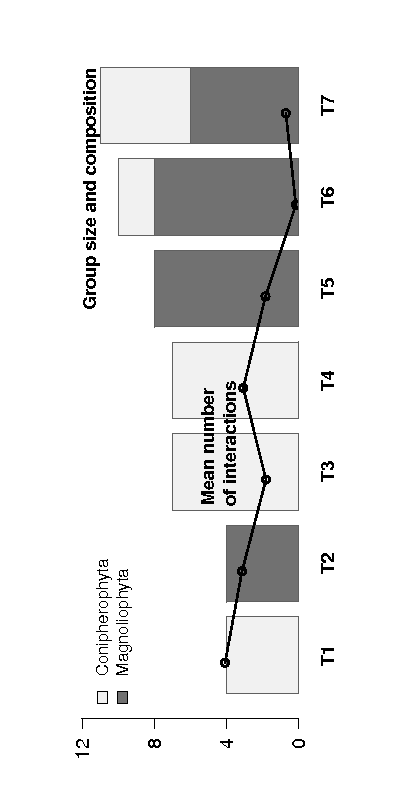
\includegraphics[height=.2\textwidth, width=.3\textwidth, trim=150 200 150 200, clip=]{\fignet/MRV10_AoAS_Q7_group}
  \end{tabular}
  
}

%====================================================================
\frame{\frametitle{Accounting for covariates} 

  \bigskip
  \paragraph{Poisson SBM with covariates.} 
  \begin{itemize}
    \item $x_{ij} =$ \emphase{taxonomic distance} between species $i$ and $j$
    \item if species $i$ belongs to cluster $k$ and species $j$ to cluster $\ell$, the number of shared parasites has a Poisson distribution with parameter $\lambda_{k\ell}$:
    $$
    (Y_{ij} \mid Z_i = k, Z_j = \ell)\sim \Pcal(e^{\alpha_{k\ell} + \beta x_{ij}})
    $$
  \end{itemize}

  \bigskip \pause
  \paragraph{Model with covariates.}  $\widehat{K} = 4$ clusters, $\widehat{\beta} = - .317$ \\ ~\\
  \begin{tabular}{ccc}
    Adjacency matrix & Clustered matrix & Clade composition \\
    \includegraphics[height=.25\textwidth, trim=0 0 0 50, clip=]{\fignet/Tree-adjMat} &
    \includegraphics[height=.25\textwidth, trim=0 0 0 50, clip=]{\fignet/Tree-adjMat-SBMtaxo}
    &
    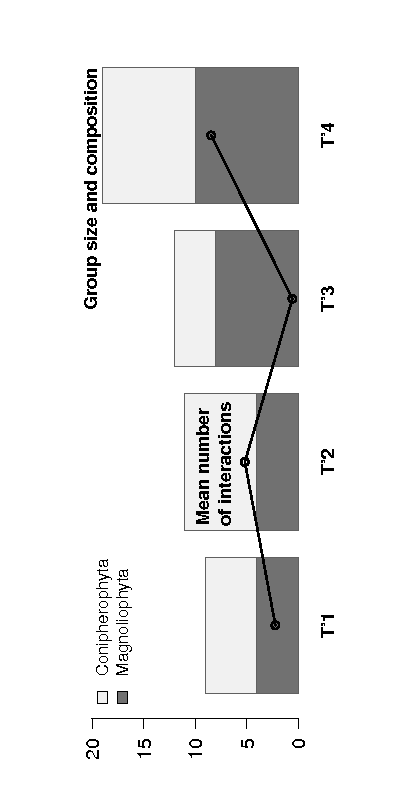
\includegraphics[height=.2\textwidth, width=.3\textwidth, trim=150 200 150 200, clip=]{\fignet/MRV10_AoAS_Q4_group}
  \end{tabular}
  
}



%====================================================================
%====================================================================
\section{Some statistical issues}
\frame{\frametitle{Outline} \tableofcontents[currentsection]}
%====================================================================
\subsection{Latent variable models}
%====================================================================
\frame{\frametitle{Latent variable models} 

  \bigskip 
  \begin{tabular}{cc}
    \hspace{-.04\textwidth}
    \begin{tabular}{p{.5\textwidth}}
      \paragraph{Latent variable model.} Three ingredients
      \begin{itemize}
        \setlength{\itemsep}{0.5\baselineskip}
        \item $Y =$ observed variables (data)
        \item $X =$ covariates (observed)
        \item $\theta =$ model parameters (unknown)
        \item $Z =$ latent variables (unobserved)
      \end{itemize}
    \end{tabular}
    &
    \begin{tabular}{p{.45\textwidth}}
      \begin{tabular}{p{.6\textwidth}}
        \begin{tikzpicture}
  \node[observed] (X) at (-1*\edgeunit, 1*\edgeunit) {$X$};
  \node[hidden] (Z) at (0*\edgeunit, 1*\edgeunit) {$Z$};
  \node[hidden] (theta) at (1*\edgeunit, 1*\edgeunit) {$\theta$};
  \node[observed] (Y) at (0, 0) {$Y$};

  \draw[dashedarrow] (X) to (Z);
  \draw[arrow] (theta) to (Z);
  \draw[arrow] (X) to (Y);
  \draw[arrow] (Z) to (Y);
  \draw[arrow] (theta) to (Y);
\end{tikzpicture}

      \end{tabular}
    \end{tabular}
  \end{tabular}

  \bigskip \pause
  \paragraph{Examples.} 
  \begin{itemize}
    \setlength{\itemsep}{0.5\baselineskip}
    \item Poisson log-normal model (PLN)
    $$
    Z_i = \text{Gaussian vector associated with site $i$}
    $$
    (encodes species dependencies) \\ ~
    \pause
    \item Stochastic block model (SBM)
    $$
    Z_i = \text{cluster to which species $i$ belongs}
    $$
    (encodes network structure)
  \end{itemize}
  
}

%====================================================================
\frame{\frametitle{Statistical issue} 

  \paragraph{Maximum likelihood inference.} Intractable likelihood (need to integrate over $Z$)
  $$
  p_\theta(Y) = \int p_\theta(Y \mid Z) p_\theta(Z) \d Z 
  $$
  while $p_\theta(Z)$ and $p_\theta(Y \mid Z)$ are easy to evaluate

  \bigskip \bigskip \pause
  \paragraph{Usual approach: EM algorithm \refer{DLR77}.} 
  \begin{itemize}
    \item E step: with current $\theta^{(h)}$, determine the conditional distribution
    $$
    p_{\theta^{(h)}}(Z \mid Y)
    $$
    \item M step: update $\theta^{(h+1)}$ as
    $$
    \theta^{(h+)} = \arg\max_\theta \Esp_{\theta^{(h)}}\left[\log p_\theta(Z \mid Y) \mid Y\right]
    $$
  \end{itemize}

}

%====================================================================
\subsection{Variational inference}
%====================================================================
\frame{\frametitle{Variational inference} 

  \paragraph{For both PLN and SBM.} Intractable E step: 
  $$
  \text{no close form or clever way to evaluate } p_{\theta^{(h)}}(Z \mid Y)
  $$
  
  \bigskip \bigskip \pause
  \paragraph{Variational inference \refer{BKM17}.} Approximate it
  $$
  q_{\psi^{(h)}(Z)} \simeq p_{\theta^{(h)}}(Z \mid Y)
  $$
  with a well chosen distribution $q_\psi \in \Qcal$ (\refer{DPR08} for SBM, \refer{CMR18a} for PLN)
  
  \bigskip \bigskip \pause
  \paragraph{Consequence.} Loose MLE properties
  \begin{itemize}
    \item consistency: $\widehat{\theta}_n \to \theta^*$
    \item asymptotic normality $\widehat{\theta}_n \approx \Ncal(\theta^*, \Var(\widehat{\theta}_n))$ (inc. confidence intervals)
    \item model selection criteria (AIC, BIC, ...)
    \item ...
  \end{itemize}

}



%====================================================================
%====================================================================
\section{Discussion}
\frame{\frametitle{Outline} \tableofcontents[currentsection]}
%====================================================================
\frame{\frametitle{Statistics for networks}

  \bigskip 
  \paragraph{Networks} are specific objects that require specific statistical models
  $$
  \text{$\to$ Make sure that the question is a network question}
  $$
  
  \bigskip \pause
  \paragraph{In practice,} two main cases
  \begin{enumerate}
    \item Pb 1: the network is unknown and needs to be inferred \\
    $\to$ $\Gcal$ is part of the model parameters
    $$
    Y \sim \Fcal(X, \theta, \Gcal)
    $$
    \item Pb 2: the network is observed and its structure needs to be understood \\
    $\to$ $\Gcal$ is the object to be modelled
    $$
    \Gcal = Y \sim \Fcal(X, \theta)
    $$
  \end{enumerate}
  
  \bigskip \pause
  \paragraph{'Complex' models} require specific inference strategies  
  \begin{itemize}
    \item variational approximations yields estimates with uncertain statistical guaranties
    \item Monte-Carlo integration yields computationally demanding algorithm \refer{TOA20}
  \end{itemize}

}

%====================================================================
\frame{\frametitle{Extensions}

  \bigskip 
  \paragraph{Modelling.} Problems 1 and 2 can be combined
  \begin{itemize}
    \item First infer $\Gcal$ from abundance data $Y$, then pose a model on $\widehat{\Gcal}$ \\
    $$
    \text{$\to$ need to be very (very (very)) careful about the uncertainty on $\widehat{\Gcal}$}
    $$
    \item Design a specific modelling, e.g. \refer{ACM09,ToC25}
    $$
    \Gcal \sim SBM(X, \theta), \qquad Y \mid \Gcal \sim PLN(X, \theta', \Gcal)
    $$
    and design the corresponding inference algorithm
  \end{itemize}

  \bigskip \bigskip \pause
  \paragraph{Statistical inference.} 
  'Post-processing' can be designed to get estimates associated with statistical guaranties
  \begin{itemize}
    \item Sequential Monte-Carlo for SBM \refer{DoR21}
    \item Importance sampling + composiste likelihood for PLN \refer{StR24}
  \end{itemize}


}


%====================================================================
%====================================================================
\backupbegin 
\section*{Backup}
%====================================================================
\frame[allowframebreaks]{ \frametitle{References}
  {%\footnotesize
   \tiny
   \bibliography{/home/robin/Biblio/BibGene}
%    \bibliographystyle{/home/robin/LATEX/Biblio/astats}
   \bibliographystyle{alpha}
  }
}

%==================================================================
\frame{\frametitle{Latent network}

  \paragraph{Some undesirable property:} {all latent (GGM) models} infer the dependency struture of the latent $Z$, not of the observed abundances $Y$
  
  \bigskip \bigskip 
  \renewcommand{\nodesize}{2em}
  \begin{overprint}
    \onslide<2>
    $$
    \begin{array}{ccc}
    p(Z, Y) & & p(Y) \\ ~\\
      \begin{tikzpicture}[scale=.8]
  \node[hidden] (Z1) at ( 0.95*\edgeunit,  0.31*\edgeunit) {$Z_1$};
  \node[hidden] (Z2) at (-0.00*\edgeunit,  1.00*\edgeunit) {$Z_2$};
  \node[hidden] (Z3) at (-0.95*\edgeunit,  0.31*\edgeunit) {$Z_3$};
  \node[hidden] (Z4) at (-0.59*\edgeunit, -0.81*\edgeunit) {$Z_4$};
  \node[hidden] (Z5) at ( 0.59*\edgeunit, -0.81*\edgeunit) {$Z_5$};
  
  \draw[edge] (Z1) to (Z5);  \draw[edge] (Z2) to (Z3);  
  \draw[edge] (Z2) to (Z4);  \draw[edge] (Z3) to (Z4); 

  \node[observed] (Y1) at ( 1.05*\edgeunit, -0.39*\edgeunit) {$Y_1$};
  \node[observed] (Y2) at (-0.00*\edgeunit,  0.30*\edgeunit) {$Y_2$};
  \node[observed] (Y3) at (-1.05*\edgeunit, -0.39*\edgeunit) {$Y_3$};
  \node[observed] (Y4) at (-0.59*\edgeunit, -1.51*\edgeunit) {$Y_4$};
  \node[observed] (Y5) at ( 0.59*\edgeunit, -1.51*\edgeunit) {$Y_5$};
  
  \draw[arrow] (Z1) to (Y1); 
  \draw[arrow] (Z2) to (Y2);
  \draw[arrow] (Z3) to (Y3);
  \draw[arrow] (Z4) to (Y4);
  \draw[arrow] (Z5) to (Y5);
  \end{tikzpicture}

    & \qquad \qquad &
      \begin{tikzpicture}[scale=.8]
  \node[observed] (Y1) at ( 0.95*\edgeunit,  0.31*\edgeunit) {$Y_1$};
  \node[observed] (Y2) at (-0.00*\edgeunit,  1.00*\edgeunit) {$Y_2$};
  \node[observed] (Y3) at (-0.95*\edgeunit,  0.31*\edgeunit) {$Y_3$};
  \node[observed] (Y4) at (-0.59*\edgeunit, -0.81*\edgeunit) {$Y_4$};
  \node[observed] (Y5) at ( 0.59*\edgeunit, -0.81*\edgeunit) {$Y_5$};
  \node[empty] (YY) at ( 0.59*\edgeunit, -1.51*\edgeunit) {};

  \draw[edge] (Y1) to (Y5);  \draw[edge] (Y2) to (Y3);  
  \draw[edge] (Y2) to (Y4);  \draw[edge] (Y3) to (Y4);  
  
  \end{tikzpicture}

    \end{array}
    $$
    \onslide<3>
    $$
    \begin{array}{ccc}
    p(Z, Y) & & p(Y) \\ ~\\
      \begin{tikzpicture}[scale=.8]
    \node[hidden] (Z1) at ( 0.95*\edgeunit,  0.31*\edgeunit) {$Z_1$};
    \node[hidden] (Z2) at (-0.00*\edgeunit,  1.00*\edgeunit) {$Z_2$};
    \node[hidden] (Z3) at (-0.95*\edgeunit,  0.31*\edgeunit) {$Z_3$};
    \node[hidden] (Z4) at (-0.59*\edgeunit, -0.81*\edgeunit) {$Z_4$};
    \node[hidden] (Z5) at ( 0.59*\edgeunit, -0.81*\edgeunit) {$Z_5$};
    
    \draw[edge] (Z1) to (Z2);  \draw[edge] (Z1) to (Z4);  
    \draw[edge] (Z1) to (Z5);  \draw[edge] (Z2) to (Z3);  
    \draw[edge] (Z2) to (Z4);  \draw[edge] (Z3) to (Z4); 

    \node[observed] (Y1) at ( 1.05*\edgeunit, -0.39*\edgeunit) {$Y_1$};
    \node[observed] (Y2) at (-0.00*\edgeunit,  0.30*\edgeunit) {$Y_2$};
    \node[observed] (Y3) at (-1.05*\edgeunit, -0.39*\edgeunit) {$Y_3$};
    \node[observed] (Y4) at (-0.59*\edgeunit, -1.51*\edgeunit) {$Y_4$};
    \node[observed] (Y5) at ( 0.59*\edgeunit, -1.51*\edgeunit) {$Y_5$};

    \draw[arrow] (Z1) to (Y1); 
    \draw[arrow] (Z2) to (Y2);
    \draw[arrow] (Z3) to (Y3);
    \draw[arrow] (Z4) to (Y4);
    \draw[arrow] (Z5) to (Y5);
  \end{tikzpicture}

    & \qquad \qquad &
      \begin{tikzpicture}[scale=.8]
  \node[observed] (Y1) at ( 0.95*\edgeunit,  0.31*\edgeunit) {$Y_1$};
  \node[observed] (Y2) at (-0.00*\edgeunit,  1.00*\edgeunit) {$Y_2$};
  \node[observed] (Y3) at (-0.95*\edgeunit,  0.31*\edgeunit) {$Y_3$};
  \node[observed] (Y4) at (-0.59*\edgeunit, -0.81*\edgeunit) {$Y_4$};
  \node[observed] (Y5) at ( 0.59*\edgeunit, -0.81*\edgeunit) {$Y_5$};
  \node[empty] (YY) at ( 0.59*\edgeunit, -1.51*\edgeunit) {};

  \draw[edge] (Y1) to (Y2);  \draw[edge] (Y1) to (Y3);  
  \draw[edge] (Y1) to (Y4);  \draw[edge] (Y1) to (Y5);  
  \draw[edge] (Y2) to (Y3);  \draw[edge] (Y2) to (Y4); 
  \draw[edge] (Y2) to (Y5);  \draw[edge] (Y3) to (Y4);  
  \draw[edge] (Y3) to (Y5);  \draw[edge] (Y4) to (Y5);  
  \end{tikzpicture}

    \end{array}
    $$
  \end{overprint}
  \renewcommand{\nodesize}{\commonnodesize}
}

%====================================================================
\frame{\frametitle{Models for species interaction networks} 

  \begin{tabular}{cc}
    \hspace{-.04\textwidth}
    \begin{tabular}{p{.5\textwidth}}
      \paragraph{Tree species interactions \refer{VPD08}:} 
      \begin{itemize}
       \item $n = 51$ tree species
       \item $Y_{ij} =$ number of fungal parasites shared by species $i$ and $j$
       \item $x_{ij} =$ vector of similarities (taxonomic, geographic, genetic) between species $i$ and $j$
      \end{itemize}
      
      \bigskip \bigskip
      \paragraph{Questions:} 
      \begin{itemize}
       \item Is the network 'organized' in some way? \\~
       \item Do the covariate contribute to explain why species interact?
      \end{itemize}

      
%       \bigskip \bigskip 
%       \paragraph{Other types of network.} 
%       \begin{itemize}
%       \item plant-pollinator: mutualistic network (bipartite) 
%       \item predator-prey: trophic network (multipartite)
%       \end{itemize}
    \end{tabular}
    &
    \begin{tabular}{p{.45\textwidth}}
      \paragraph{Network (weighted):} \\
%       \includegraphics[height=.25\textwidth,width=.25\textwidth,trim=30 30 30 30]     
      \includegraphics[height=.3\textwidth,width=.3\textwidth]{\fignet/Tree-netCircle}
 \\
      \paragraph{Adjacency matrix (counts):} \\
      \includegraphics[height=.3\textwidth,width=.3\textwidth]{\fignet/Tree-adjMat}
    \end{tabular}
  \end{tabular}
      
}

%====================================================================
\frame{\frametitle{PLN for dimension reduction (PCA)}

  \begin{tabular}{cl}
    \hspace{-.04\textwidth}
    \begin{tabular}{p{.3\textwidth}}
      \paragraph{Metabarcoding data} \refer{JFS16} \\ ~
      \begin{itemize}
      \item $p = 114$ OTUs (bacteria and fungi) \\ ~
      \item $n = 116$ leaves \\ ~
      \item collected on 3 trees 
        \begin{itemize}
        \item resistant 
        \item intermediate
        \item susceptible       
      \end{itemize}
      to oak powdery mildew
      \end{itemize}

      \bigskip \bigskip 
      \paragraph{Model selection:} 
      \begin{itemize}
        \item Penalized lower-bound $J(\widehat{\theta}, \widehat{q})$ \\
        (pseudo BIC, pseudo ICL, \dots)
      \end{itemize}

    \end{tabular}
    &
    \begin{tabular}{p{.55\textwidth}}
    \includegraphics[height=.4\textheight]{\fignet/CMR18-AnnApplStat-Fig4a} \\
    ~ \\
    \includegraphics[height=.4\textheight]{\fignet/CMR18-AnnApplStat-Fig5a} 
    \end{tabular}
  \end{tabular}
}

%====================================================================
\frame{\frametitle{Poisson SBM with covariates: choosing $K$}

  \begin{tabular}{c|c|c}
    & & \paragraph{Including the} \\
    & \paragraph{No covariate} & \paragraph{taxonomic distance} \\
    & & \\
    Observed network & Clustering (no covariate) & Group composition \\
    \includegraphics[width=.3\textwidth]{\fignet/Tree-adjMat}
    &
    \includegraphics[width=.3\textwidth]{\fignet/Tree-adjMat-SBMnull}
    &
    \includegraphics[width=.3\textwidth]{\fignet/Tree-adjMat-SBMtaxo}
    \\
    Model selection & Clustering & Group composition \\
    \includegraphics[width=.3\textwidth,width=.25\textwidth]{\fignet/Tree-ICL-SBMall}
    &
    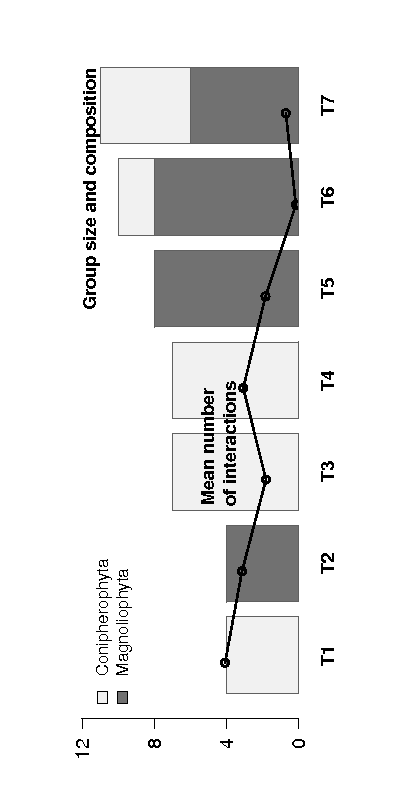
\includegraphics[width=.3\textwidth,height=.25\textwidth,trim=0 20 0 100]{\fignet/MRV10_AoAS_Q7_group}
    &
    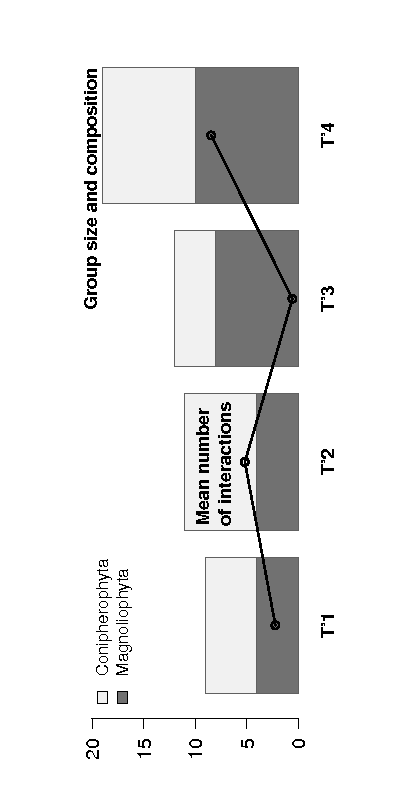
\includegraphics[width=.3\textwidth,height=.25\textwidth,trim=0 20 0 100]{\fignet/MRV10_AoAS_Q4_group}  
  \end{tabular}

}

%====================================================================
\frame{\frametitle{Tree interaction network: posterior distributions} 

  \bigskip 
  \paragraph{Do the distance between the tree species contribute to structure network?} \refer{DoR19}
  $$
  \begin{tabular}{ccc}
    taxonomy & geography & genetics \\
    \includegraphics[width=.25\textwidth]{\figbayes/Tree-all-V10-M5000-beta1} & 
    \includegraphics[width=.25\textwidth]{\figbayes/Tree-all-V10-M5000-beta2} & 
    \includegraphics[width=.25\textwidth]{\figbayes/Tree-all-V10-M5000-beta3}
  \end{tabular}
  $$
  
  \bigskip \pause
  \hspace{-.025\textwidth}
  \begin{tabular}{rrrr}
    \paragraph{Correlation between estimates.} 
    & $(\beta_1, \beta_2)$ & $(\beta_1, \beta_3)$ & $(\beta_2, \beta_3)$ \\
    $p_{VEM}(\beta)$    & $-0.012$ & $ 0.021$ & $ 0.318$ \\
    $p(\beta \mid Y)$ & $-0.274$ & $-0.079$ & $-0.088$
  \end{tabular}

  \bigskip \bigskip 
  \paragraph{Model selection.} 
  $$
  P\{X = \text{(taxo., geo.)} \mid Y \} \simeq 70\%, \qquad
  P\{X = \text{(taxo.)} \mid Y \} \simeq 30\%
  $$

}

%====================================================================
\frame{\frametitle{Fish species in the Barents sea}

  \newcommand{\figStR}{/home/robin/RECHERCHE/BAYES/PLNsampling/Paper/Figures}
  \newcommand{\nIterEx}{10000} \newcommand{\lagEx}{50} \newcommand{\nISex}{200}
  \newcommand{\exampleParms}{-nIter\nIterEx-lag\lagEx-nIS\nISex}
  \newcommand{\nIterSel}{\nIterEx} \newcommand{\lagSel}{20} \newcommand{\nISsel}{\nISex}
  \newcommand{\selectParms}{-nIS\nISsel-nIter\nIterSel-lag\lagSel}
  
  \bigskip
  \paragraph{Comparison of the estimates.} \refer{StR24}
  $$
  \begin{tabular}{ccc}
    $\widehat{B}$ & $\widehat{\Sigma}$ & ESS (CL5) \\
    \includegraphics[width=.25\textwidth, trim=10 10 25 50, clip=]{\figStR/Barents\exampleParms-compBeta-cem5-all} & 
    \includegraphics[width=.25\textwidth, trim=10 10 25 50, clip=]{\figStR/Barents\exampleParms-compSigma-cem5-all} & 
    \includegraphics[width=.25\textwidth, trim=10 10 25 50, clip=]{\figStR/Barents\exampleParms-ESS-cem5}     
  \end{tabular}
  $$

  \pause
  \paragraph{Significance.} Test statistics $\widehat{\theta} \left/ \sqrt{\widehat{\Var}_\infty(\widehat{\theta})} \right.$
  $$
  \begin{tabular}{ccc}
    $\widehat{B}$ & $\widehat{\Sigma}$ & $\text{cor}(\widehat{\Sigma})$ \\
    \includegraphics[width=.25\textwidth, trim=10 10 25 25, clip=]{\figStR/Barents\exampleParms-betaSignif-cem5} & 
    \includegraphics[width=.25\textwidth, trim=10 10 25 25, clip=]{\figStR/Barents\exampleParms-sigmaSignif-cem5} &
    \includegraphics[width=.25\textwidth, trim=10 10 25 25, clip=]{\figStR/Barents\exampleParms-corSigmaSignif-cem5}
  \end{tabular}  
  $$
}

%====================================================================
\backupend 
%====================================================================



%====================================================================
%====================================================================
\end{document}
%====================================================================
%====================================================================

  \begin{tabular}{cc}
    \hspace{-.04\textwidth}
    \begin{tabular}{p{.5\textwidth}}
    \end{tabular}
    &
    \begin{tabular}{p{.45\textwidth}}
    \end{tabular}
  \end{tabular}

